\documentclass[12pt,a4paper]{article}
\usepackage[a4paper,top=1.5cm, bottom=1.5cm, left=1.5cm, right=1.5cm]{geometry}
\usepackage[T2A]{fontenc}
\usepackage[utf8]{inputenc}
\usepackage[russian]{babel}
\usepackage{amsmath}
\usepackage{amssymb}
\usepackage{graphicx}
\usepackage{floatrow}
\usepackage{booktabs}
\usepackage{wrapfig}
\usepackage{indentfirst}
\usepackage{lipsum}
\usepackage{subcaption}
\usepackage{float}
\usepackage{enumitem}
\restylefloat{table}

\newcommand{\figref}[1]{(см. рис. \ref{#1})}
\newcommand{\e}[1]{\text{$\cdot10^{#1}$}}

\title{Лабораторная работа 5.5.5 \\ Компьютерная сцинтилляционная $\gamma$-спектрометрия}
\author{Симанкович Александр\\ Б01-108}
\date{07.10.2023}

\begin{document}
	\maketitle
	
	\section*{Аннотация}
	
	В работе экспериментально определяются спектры $\gamma$-квантов, которые формируются при распаде Co, Cs, Na, Eu, Am. Проводится анализ спектров.
	
	\section*{Теоретическое введение}
	
	\subsection*{Базовые принципы работы сцинтиллятора}
	
	При прохождении $\gamma$-квантов через среду существует три механизма взаимодействия со средой: фотоэффект, комптоновское рассеяние и образование электрон-позитронных пар. Эти эффекты приводят к образованию быстрых электронов в веществе. Быстрые электроны ионизируют и возбуждают атомы при движении через вещество за счет неупругих столкновений. При переходах атомов и молекул в основное состояние и рекомбинации излучаются фотоны, характерные для вещества сцитиллятора.
	
	Обратим внимание, что такие фотоны должны иметь очень небольшой шанс выйти из сцинтиллятора, поскольку их энергия совпадает с разностью энергий между уровнями. Поэтому кристалл (напр. NaI) легируется примесью (напр. Tl) с малой концентрацией ($0.1\%$). Примесь имеет излучающий переход в запрещенной зоне кристалла. Таким образом, фотон может без потерь двигаться сквозь кристалл.
	
	Вспышки из сцинтиллятора имеют низкую интенсивность, для усиления используется фотоэлектронный умножитель. С помощью фотоэффекта и электронной лавины сигнал усиливается, после чего передается на АЦП.
	
	\subsection*{Процессы взаимодействия $\gamma$-излучения с веществом}
	
	\subsubsection*{Фотоэффект}
	
	Процесс поглощения $\gamma$-кванта связанным электроном. Электрон получает почти всю энергию $\gamma$-кванта, часть которой затрачивается на потенциал ионизации:
	$$T_e = E_{\gamma} - I_i.$$
	Более вероятен для тяжелых веществ и низкоэнергетичных фотонов.
	
	\subsubsection*{Комптоновское рассеяние}
	
	Рассеяние фотона на свободном электроне. Электрон получает часть энергии $\gamma$-кванта. Максимальная возможная энергия электрона:
	\begin{equation}
		E_{max} = \frac{\hbar \omega}{1 + \frac{mc^2}{2\hbar \omega}}.
		\label{eq:compton}
	\end{equation}
	
	\subsubsection*{Образование электрон-позитронных пар}
	
	Энергия кванта идет на образование пары электрон-позитрон. Данное явление происходит в присутствии ядра или электрона, поскольку в пустоте законы сохранения для электрон-позитронной пары несовместны. Пороговая энергия:
	$$ E_{\text{пор}} = 2mc^2 = 1.022 \text{ МэВ}.$$
	
	Образовавшийся электрон будет двигаться, теряя энергию на ионизацию и возбуждение атомов. Его энергия полностью останется в детекторе. Позитрон аннигилирует с электроном, излучив два $\gamma$-кванта. Один или оба $\gamma$-кванта могут покинуть детектор.
	
	\subsection*{Компоненты спектра}
	
	В спектре будут наблюдаться различные составляющие:
	
	1. \textit{Фотопик}. Формируется при рассеянии полной энергии начального $\gamma$-кванта.
	
	2. $E_{\gamma} - E_0, E_{\gamma} - 2 E_0$. Компоненты от электрон-позитронных пар.
	
	3. \textit{Пик обратного рассеяния}. Формируется от рассеяния $\gamma$-квантов от стенок детектора. Положение пика:
	\begin{equation}
		E_{\text{обр}} =	\frac{E}{1 + 2E / mc^2}.
		\label{eq:backscattering}
	\end{equation}
	
	4. \textit{Комптоновский спектр}. Континуальный спектр от комптоновского рассеяния.
	
	\subsection*{Энергетическое разрешение спектрометра}
	
	При поглощении частиц с одинаковой энергии, значения энергии, получаемые спектрометром, будут различаться. Это связано со статистической природой сцинтиллятора. Как следствие, пик, который должен быть $\delta$-функцией, становится размытым.
	
	Энергетическое разрешение спектрометра:
	$$R_i = \frac{\Delta E_i}{E_i},$$
	где $E_i$ -- положение пика, $\Delta E_i$ -- ширина пика на половине его высоты.
	
	Получим оценку для $R_i$. Энергия $E_i$ пропорциональна среднему числу фотонов $\overline{n_i}$:
	$$E_i = \alpha \overline{n_i}.$$
	
	Ширина пика $\Delta E_i$ пропорциональна дисперсии $\overline{\Delta n_i}$. При этом $\overline{\Delta n_i} \approx \sqrt{\overline{n_i}}$, если приблизить форму пика гауссианом.
	
	Тогда для $R_i$:
	\begin{equation}
		R_i = \frac{\Delta E_i}{E_i} = \frac{const}{\sqrt{E_i}}.
		\label{eq:R_i}
	\end{equation}

	\section*{Методика эксперимента}

	\begin{figure}[H]
		\centering
		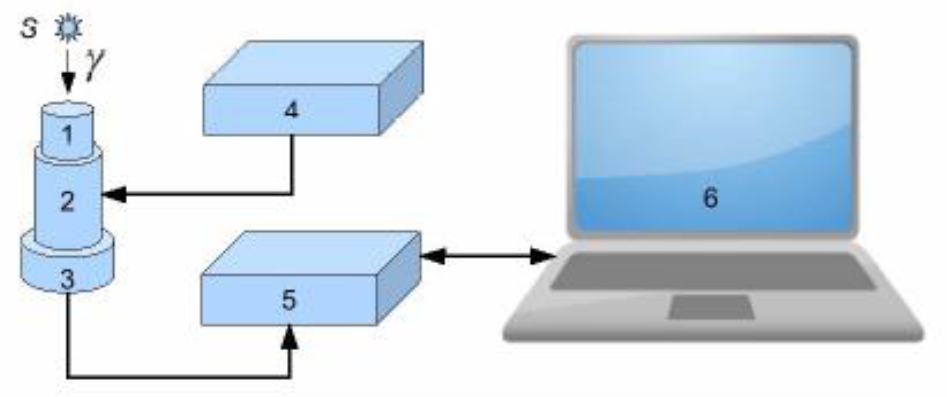
\includegraphics[scale=0.5]{res/scheme.png}
		\caption{\centering
				 Принципиальная схема спектрометра.
				 (S - источник $\gamma$-квантов, 1 - сцинтиллятор, 2 - ФЭУ, 3 - предусилитель импульсов, 4 - блок питания ФЭУ, 5 - АЦП, 6 - компьютер для сбора и обработки данных)}
		\label{fig:scheme}
	\end{figure}
	
	Принципиальная схема приведена на рис. \ref{fig:scheme}. В качестве сцинтиллятора используется кристалл NaI(Tl). Сцинтиллятор, усилитель и источник излучения находятся в защитном кожухе, предохраняющем от внешнего излучения. Сигнал с ФЭУ усиливается и подается на АЦП, после чего сохраняется на компьютере. Обработанный сигнал выводится на экран в виде графика спектра.
		
	\section*{Результаты}
	
	\subsection*{Кобальт $^{60}$Co}

	Кобальт $^{60}_{27}$Co претерпевает $\beta^{-}$ распад в $^{60}_{28}$Ni по двум схемам. После этого излучается один или два $\gamma$-кванта. Энергии указаны на схеме (\ref{fig:co_scheme}).

	\begin{figure}[H]
		\centering
		\begin{minipage}{0.55\textwidth}
				\centering
				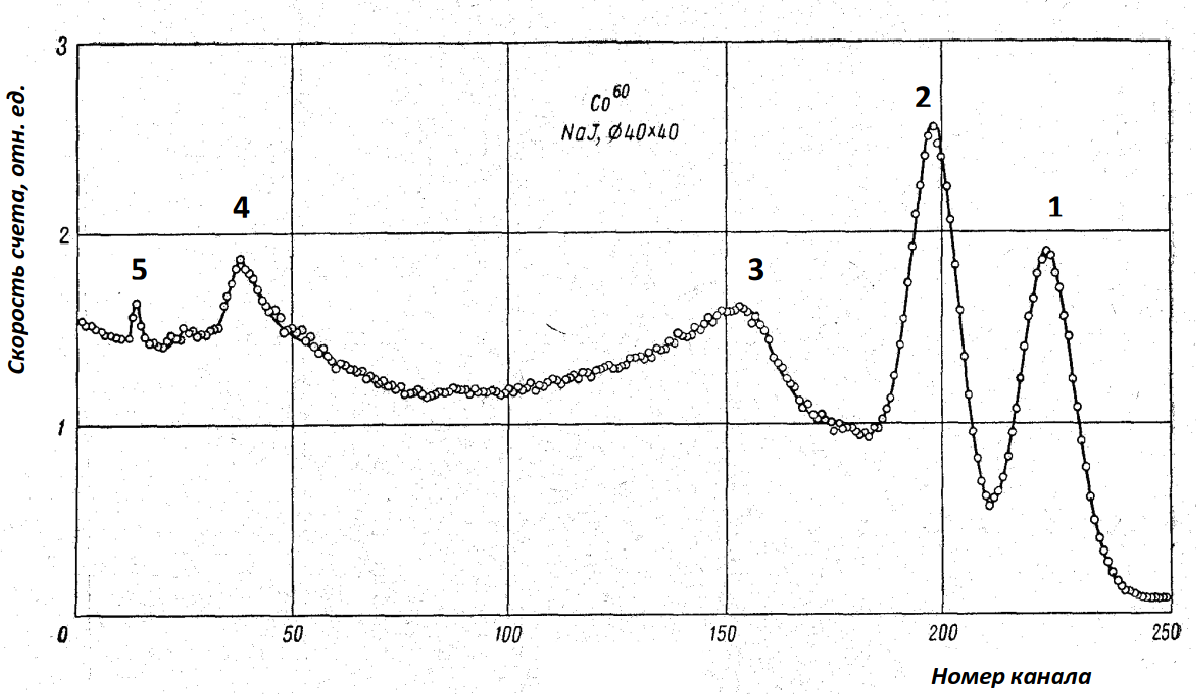
\includegraphics[width=0.9\linewidth]{res/co_spectre.png}
			\end{minipage}%
		\begin{minipage}{0.45\textwidth}
				\centering
				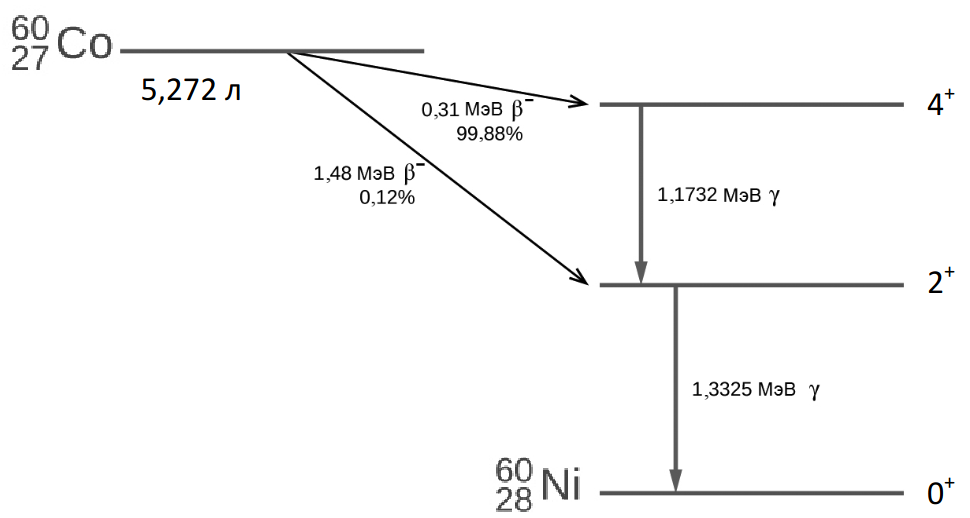
\includegraphics[width=1.0\linewidth]{res/co_levels.png}
			\end{minipage}
		\caption{\centering
				Слева: спектр $^{60}$Co (1,2 - фотопики, 3 - край комптоновского спектра, 4 - пик обратного рассеяния, 5 - пик характеристического излучения свинца). \newline
				Справа: схема распада $^{60}$Co.}
		\label{fig:co_scheme}
	\end{figure}
	
	
	\begin{figure}[H]
		\centering
		\begin{minipage}{0.5\textwidth}
			\centering
			\includegraphics[width=1.0\linewidth]{gen/co60.pdf}
		\end{minipage}%
		\begin{minipage}{0.5\textwidth}
			\centering
			\includegraphics[width=1.0\linewidth]{gen/co60_log.pdf}
		\end{minipage}
		\caption{Измеренный спектр $^{60}$Co}
		\label{fig:co_spectrum}
	\end{figure}
		
	\subsection*{Цезий $^{137}$Cs}
	
	
	Ядро $^{137}_{55}$Cs испытывает $\beta^{-}$ распад, в результате которого образует-
	ся ядро $^{137}_{56}$Ba. Большинство переходов происходит на возбужденный метастабильный уровень ядра. При переходе в основное состояние излучается $\gamma$-квант.
	
	\begin{figure}[H]
		\centering
		\begin{minipage}{0.55\textwidth}
			\centering
			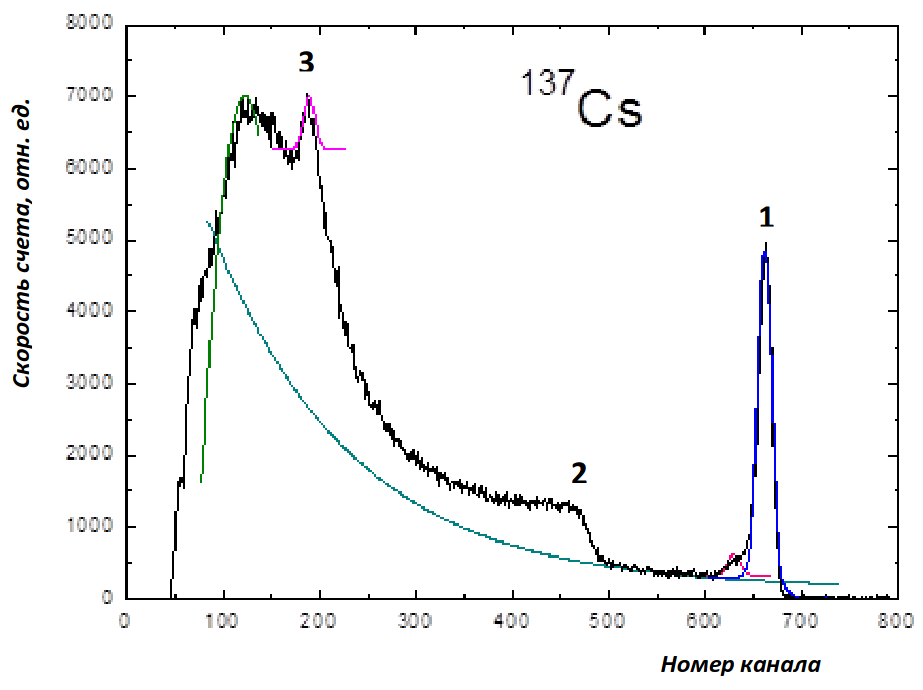
\includegraphics[width=0.9\linewidth]{res/cs_spectre.png}
		\end{minipage}%
		\begin{minipage}{0.45\textwidth}
			\centering
			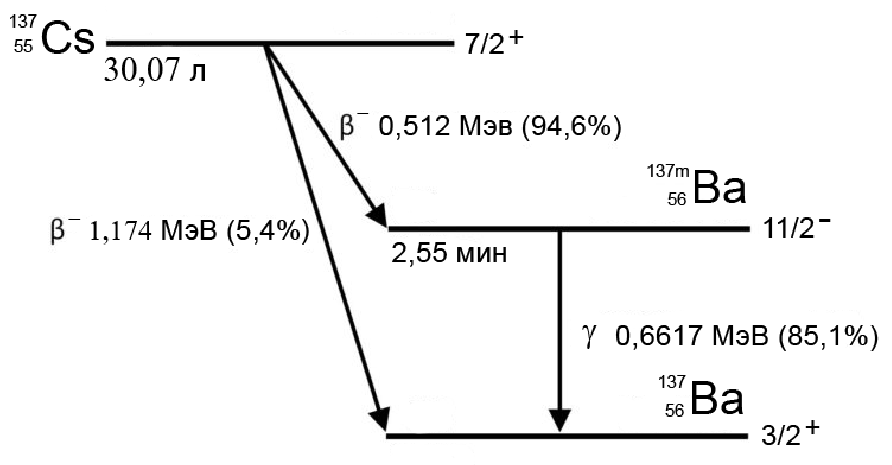
\includegraphics[width=1.0\linewidth]{res/cs_levels.png}
		\end{minipage}
		\caption{\centering
			Слева: спектр $^{137}$Cs (1 - фотопик, 2 - край комптоновского спектра, 3 - пик обратного рассеяния).
			Справа: схема распада $^{137}$Cs.}
		\label{fig:cs_scheme}
	\end{figure}
	
	\begin{figure}[H]
		\centering
		\begin{minipage}{0.5\textwidth}
			\centering
			\includegraphics[width=1.0\linewidth]{gen/cs137.pdf}
		\end{minipage}%
		\begin{minipage}{0.5\textwidth}
			\centering
			\includegraphics[width=1.0\linewidth]{gen/cs137_log.pdf}
		\end{minipage}
		\caption{Измеренный спектр $^{137}$Cs}
		\label{fig:cs_spectrum}
	\end{figure}
	
	
	\subsection*{Натрий $^{22}$Na}
	
	Вещество $^{22}$Na подвержено, в отличие от $^{60}$Co и $^{137}$Cs, $\beta^{+}$ распаду. Позитроны аннигилируют, не долетая до сцинтиллятора, давая $\gamma$-кванты, долетающие до сцинтиллятора и дающие аннигиляционный пик 511 кэВ. Также есть фотопик от перехода в основное состояние.
	
	\begin{figure}[H]
		\centering
		\begin{minipage}{0.55\textwidth}
			\centering
			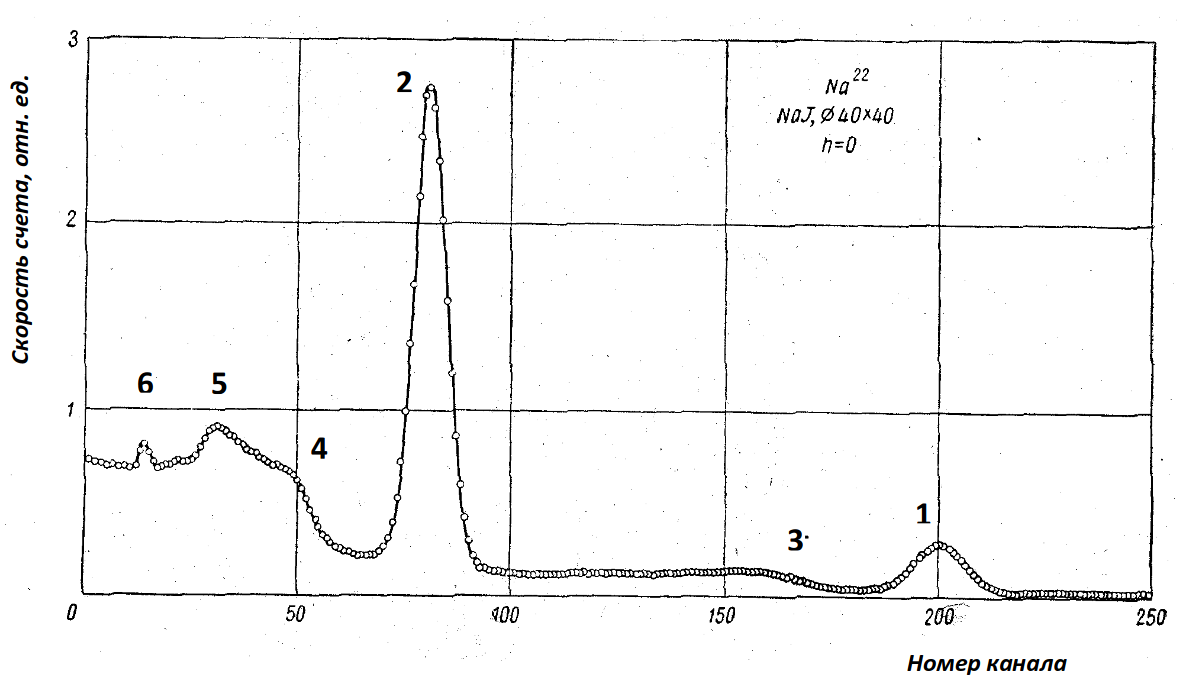
\includegraphics[width=0.9\linewidth]{res/na_spectre.png}
		\end{minipage}%
		\begin{minipage}{0.45\textwidth}
			\centering
			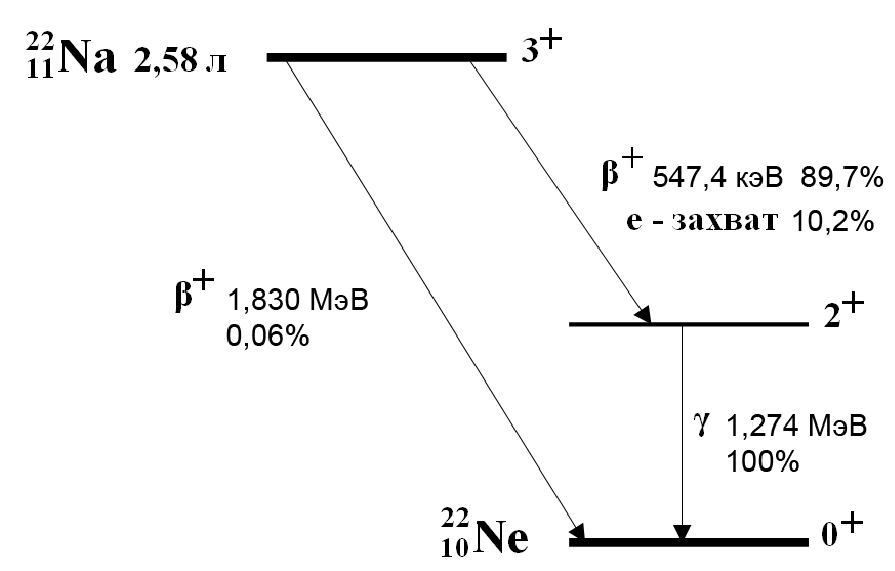
\includegraphics[width=1.0\linewidth]{res/na_levels.png}
		\end{minipage}
		\caption{\centering
			Слева: спектр $^{22}$Na (1 - фотопик, 2 - аннигиляционный пик, 3,4 - края комптоновских спектров, 5 - пик обратного рассеяния, 6 - пик характеристического излучения свинца). \newline
			Справа: схема распада $^{22}$Na.}
		\label{fig:na_scheme}
	\end{figure}
	
	
	\begin{figure}[H]
		\centering
		\begin{minipage}{0.5\textwidth}
			\centering
			\includegraphics[width=1.0\linewidth]{gen/na22.pdf}
		\end{minipage}%
		\begin{minipage}{0.5\textwidth}
			\centering
			\includegraphics[width=1.0\linewidth]{gen/na22_log.pdf}
		\end{minipage}
		\caption{Измеренный спектр $^{22}$Na}
		\label{fig:na_spectrum}
	\end{figure}
	
	
	\subsection*{Европий $^{152}$Eu}
	
%	Вещество $^{22}$Na подвержено, в отличие от $^{60}$Co и $^{137}$Cs, $\beta^{+}$ распаду. Позитроны аннигилируют, не долетая до сцинтиллятора, давая $\gamma$-кванты, долетающие до сцинтиллятора и дающие аннигиляционный пик 511 кэВ. Также есть фотопик от перехода в основное состояние.
	
	% Первый пик может быть обратным отражением
	
	\begin{figure}[H]
		\centering
		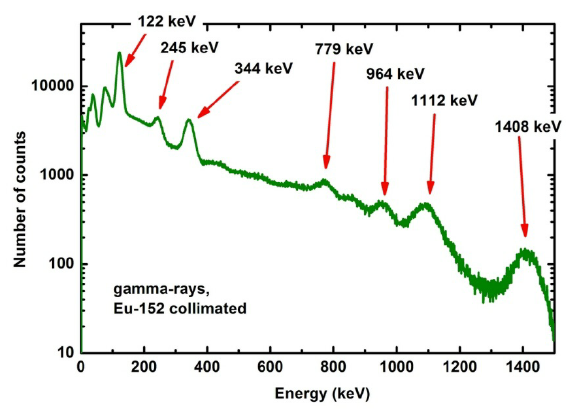
\includegraphics[width=0.7\linewidth]{res/eu_spectre.png}
		\caption{Спектр $^{152}$Eu}
		\label{fig:eu_ref_spectrum}
	\end{figure}
		
	\begin{figure}[H]
		\centering
		\begin{minipage}{0.5\textwidth}
			\centering
			\includegraphics[width=1.0\linewidth]{gen/eu152.pdf}
		\end{minipage}%
		\begin{minipage}{0.5\textwidth}
			\centering
			\includegraphics[width=1.0\linewidth]{gen/eu152_log.pdf}
		\end{minipage}
		\caption{Измеренный спектр $^{152}$Eu}
		\label{fig:eu_spectrum}
	\end{figure}
	
	\subsection*{Америций $^{241}$Am}
	
	\begin{figure}[H]
		\centering
		\begin{minipage}{0.5\textwidth}
			\centering
			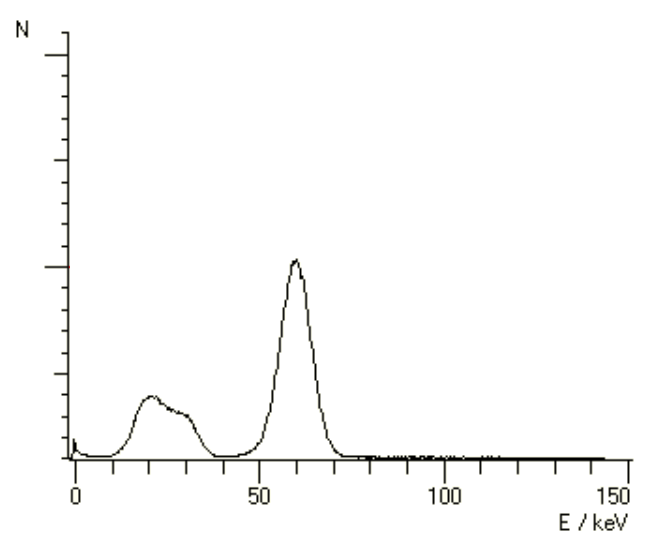
\includegraphics[width=0.9\linewidth]{res/am_spectre.png}
		\end{minipage}%
		\begin{minipage}{0.5\textwidth}
			\centering
			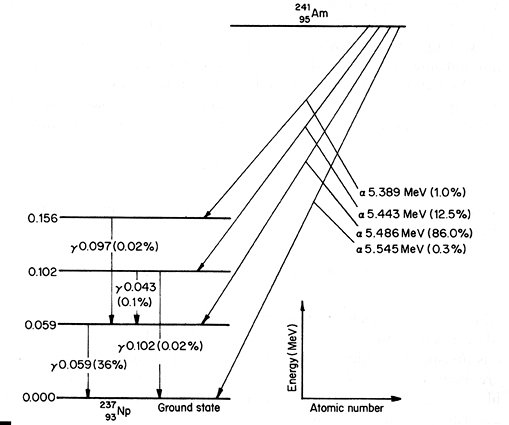
\includegraphics[width=1.0\linewidth]{res/am_scheme.jpg}
		\end{minipage}
		\caption{\centering
			Слева: спектр $^{241}$Am.
			Справа: схема распада $^{241}$Am.}
		\label{fig:am_scheme}
	\end{figure}
	
	%	Вещество $^{22}$Na подвержено, в отличие от $^{60}$Co и $^{137}$Cs, $\beta^{+}$ распаду. Позитроны аннигилируют, не долетая до сцинтиллятора, давая $\gamma$-кванты, долетающие до сцинтиллятора и дающие аннигиляционный пик 511 кэВ. Также есть фотопик от перехода в основное состояние.
	
	% Первый пик может быть обратным отражением
					
	\begin{figure}[H]
		\centering
		\begin{minipage}{0.5\textwidth}
			\centering
			\includegraphics[width=1.0\linewidth]{gen/am241.pdf}
		\end{minipage}%
		\begin{minipage}{0.5\textwidth}
			\centering
			\includegraphics[width=1.0\linewidth]{gen/am241_log.pdf}
		\end{minipage}
		\caption{Измеренный спектр $^{241}$Am}
		\label{fig:am_spectrum}
	\end{figure}
		
	\subsection*{Калибровка каналов спектрометра}
	
	Откалибруем спектрометр по известным нам энергиям некоторых пиков.
	
	\begin{table}[H]
		\input{gen/calibration.tex}
		\caption{Пики для калибровки}
	\end{table}
	
	\begin{figure}[H]
		\centering
		\includegraphics[scale=1.0]{gen/calibration.pdf}
		\caption{Калибровочная прямая}
		\label{fig:calibration}
	\end{figure}
	
	\subsection*{Фотопики}
	С помощью калибровки пересчитаем значения положений фотопиков и их ширины.

	\begin{table}[H]
		\input{gen/photopeaks.tex}
		\caption{Характеристики фотопиков}
	\end{table}
	
	Проверим зависимость \eqref{eq:R_i}. Построим $R_i^2 = f(1/E_i)$.
	
	\begin{figure}[H]
		\centering
		\includegraphics[scale=1.0]{gen/R_i.pdf}
		\caption{Линеаризация разрешения $R_i$ от энергии $E_i$}
		\label{fig:R_i}
	\end{figure}
	
	\newpage
	\subsection*{Обратное рассеяние}
	
	Некоторые пики на спектре вызваны обратным рассеянием. Построим таблицу для всех пиков:
	
	\begin{table}[H]
		\footnotesize
		\input{gen/back.tex}
		\caption{Характеристики всех пиков}
	\end{table}
	
	Пики вызванные обратным рассеянием обозначены как $(back)$, фотоэффектом -- $(photo)$, аннигиляцией -- $(annih)$, характеристическое излучение свинца -- $(pb)$.
	
	Большинство пиков для европия предполагаются 
	
	
	\subsection*{Комптоновский спектр}
	
	Пересчитаем значения энергии на краях комптоновских спектров ($E_k$). Также рассчитаем края комптоновских спектров исходя из \eqref{eq:compton} ($E_k^{theory}$).
	\begin{table}[H]
		\input{gen/compton.tex}
		\caption{Края комптоновских спектров}
	\end{table}
	
	\begin{figure}[H]
		\centering
		\includegraphics[scale=1.0]{gen/compton.pdf}
		\caption{Зависимость $E_k$ от энергии $E_k^{theory}$}
		\label{fig:E_k}
	\end{figure}
	
	Как можно видеть, теоретические значения хорошо описывают экспериментальные данные.
	
	\subsection*{Характеристическое излучение свинца}
	
	Для Co, Cs, Na на графиках можно наблюдать характеристическое излучение свинца.

	\begin{table}[H]
		\input{gen/pb.tex}
		\caption{Характеристическое излучение свинца}
	\end{table}
	
	С учетом ширины пиков получим:
	
	$$ E_{pb} = (116 \pm 10) \text{ кэВ} $$
	
	\section*{Заключение и выводы}
	
	В работе экспериментально получены спектры $\gamma$-квантов, образующихся при распаде Co, Cs, Na, Eu, Am. Проведен анализ спектров. Вычислено значение энергии характеристического излучения свинца $E_{pb} = (116 \pm 10) \text{ кэВ}$. Проверена зависимость края комптоновского излучения от энергии фотопика.
	
	В качестве улучшения работы можно провести более тщательный анализ пиков, поскольку некоторые из них имеют неизвестное происхождение.
	
\end{document}
